\section{Experimental Results}
\label{section:experimental-results}

Many different design combinations of a reward function seem possible. This paper does not try to identify the best solution. Instead, it shows that there exists better implementations than the conventional XCS algorithm. Therefore, this paper concentrates on a comparison of XCS variants, as presented in Section~\ref{subsection:xcs-variants}. To properly compare these variants, it has been important to determine good parameter settings for each variant. While most of the standard values given in~\cite{BW02} and known as \emph{commonly used parameter settings} provide good results, some special settings need closer examination (see Section~\ref{subsection:xcs-parameters}). Thereby, thousands of different combinations have been tested and the parameter discussion could not completely presented in here. Configurations that achieved a lower performance than a simple \emph{random walk} strategy are also omitted, since it is always difficult to argue, whether the increased performance of the predators' behavior is caused by an improved learning or by acting more equal to the \emph{random walk} strategy. % E.\,g., in the \emph{random scenario} with an \emph{obstacle-evading prey}, none of the investigated XCS variants have been able to show a significant better result than the \emph{random walk} strategy, so that this specific scenario has been omitted from further investigations. 
Finally, selected results % of a number of experiments 
are discussed in Section~\ref{subsection:discussion-of-experimental-results}.

% A major focus has been set on the comparison to a scenario, where predators completely behave on the base of randomized movements. Thus, all obtained results below such this random scenario have been rejected, since it is always difficult to argue, if a parameter setting with better results (and below the result of a random algorithm) just makes the predator's movements more random or if it actually learns better. The results of the parameter discussion are presented in Section~\ref{subsection:xcs-parameters}. 

\subsection{XCS Parameters}
\label{subsection:xcs-parameters}

% TODO: Bemerken, dass f�r Vergleich XCS / SXCS im difficult scenario hohe maxStackSize Werte besser sind

\begin{figure}[ht]
	\subfigure[\emph{Pillar scenario}]{ % with an \emph{ob\-sta\-cle-} and a \emph{pre\-da\-tor-evading prey}]{
		\label{figure:max-stack-size1}
		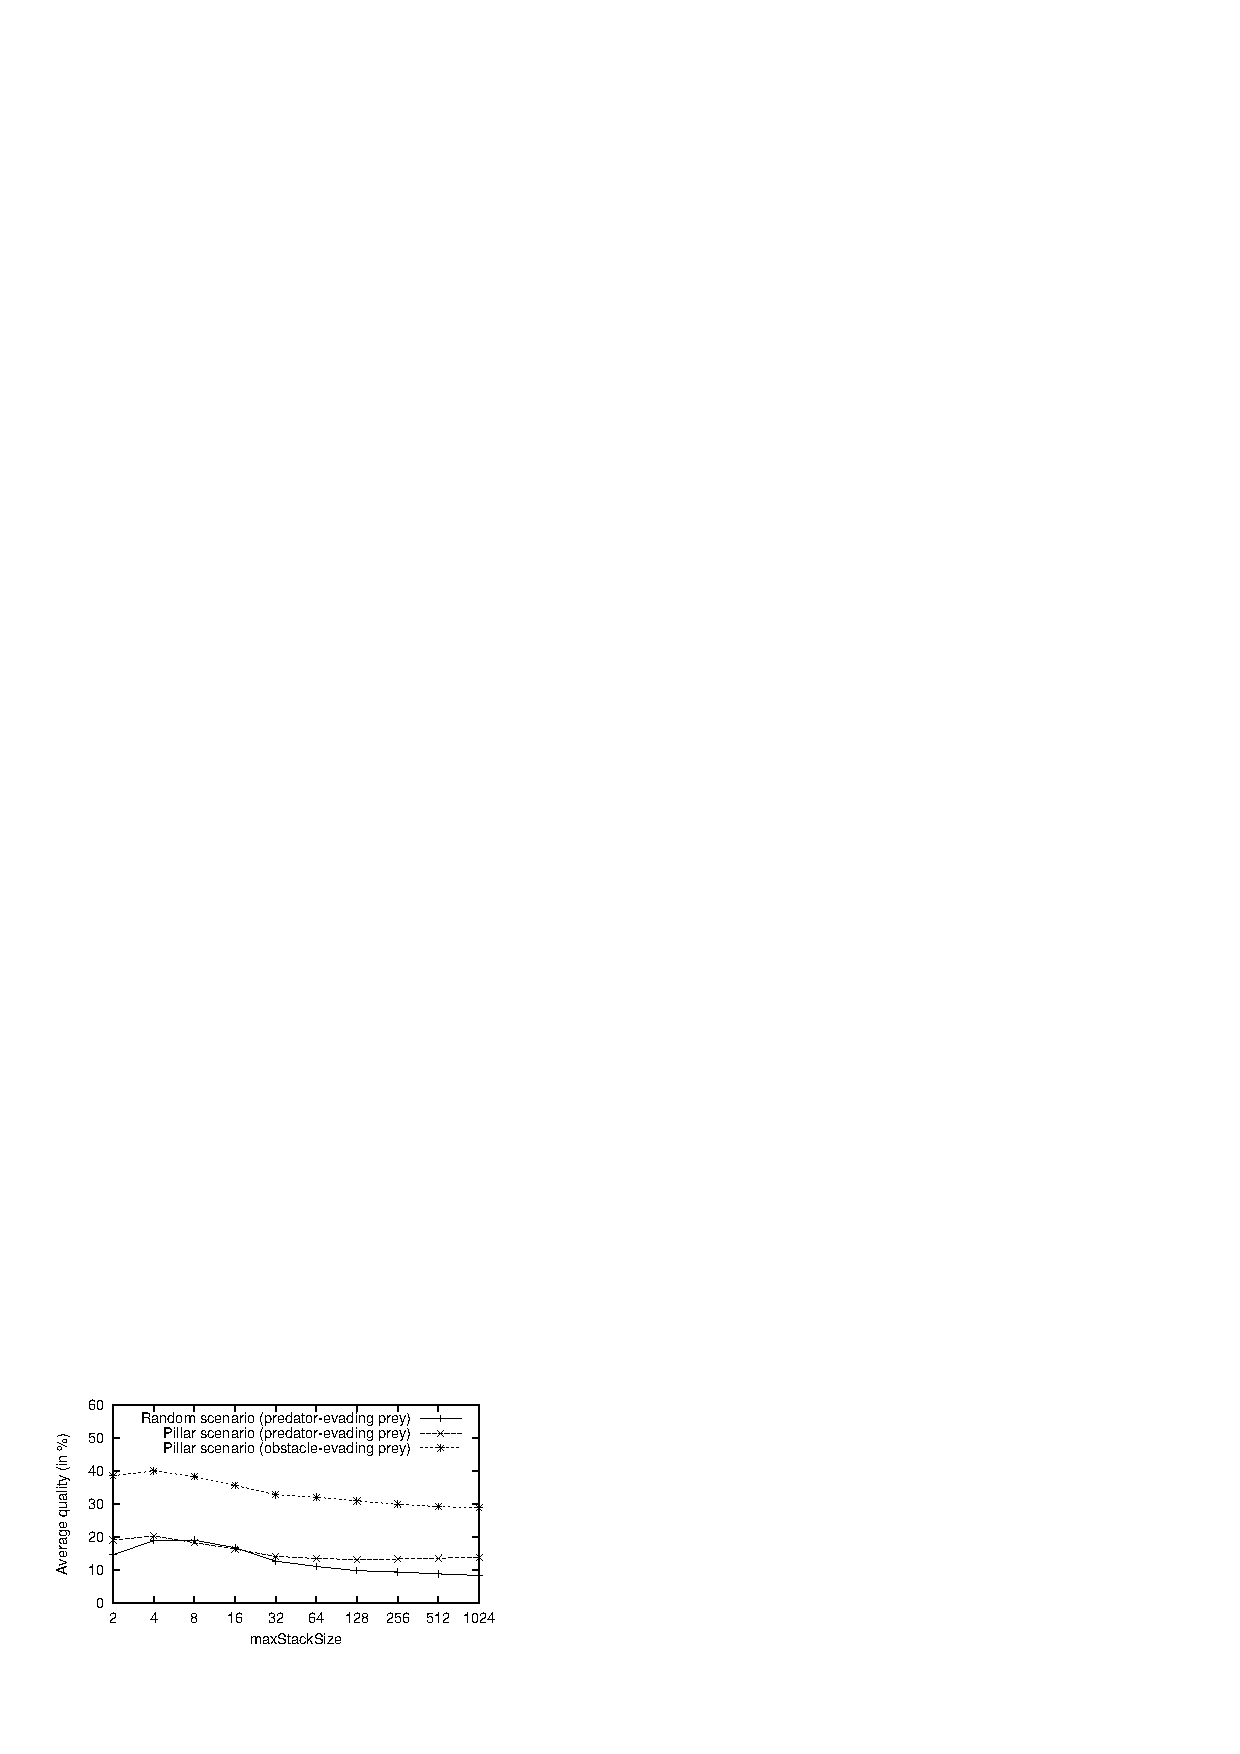
\includegraphics[width=0.15\textwidth]{plot_quality_maxstacksize1}}\hfill
	\subfigure[\emph{Random scenario}]{ % with an \emph{ob\-sta\-cle-} and a \emph{pre\-da\-tor-evading prey}]{
		\label{figure:max-stack-size2}
		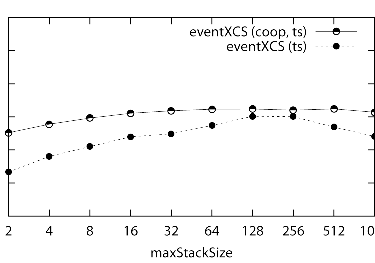
\includegraphics[width=0.15\textwidth]{plot_quality_maxstacksize2}}\hfill
	\subfigure[\emph{Difficult scenario}]{ % with a \emph{blind\-ed prey}]{
		\label{figure:max-stack-size3}
		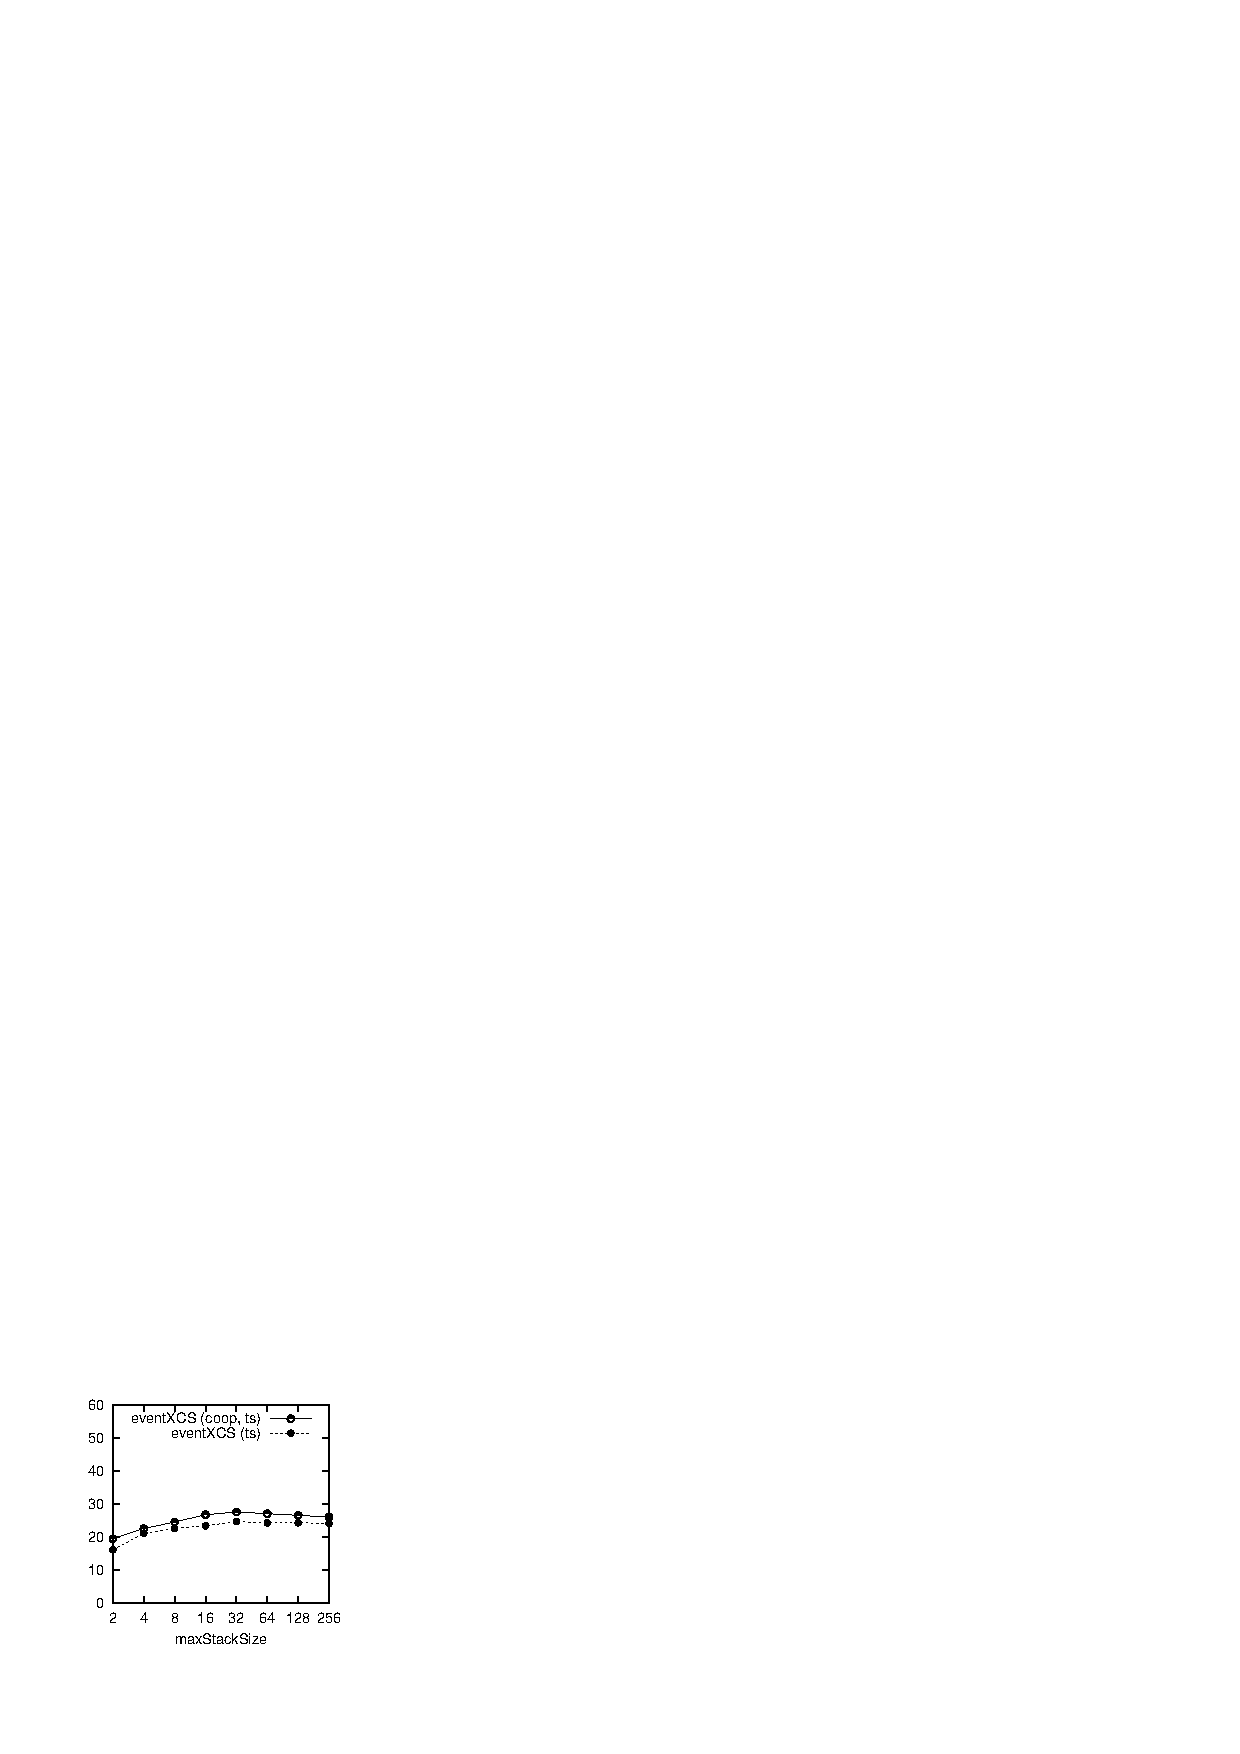
\includegraphics[width=0.15\textwidth]{plot_quality_maxstacksize3}}\hfill
	\caption{\mathversion{bold}Comparison of variants of \emph{eventXCS} with different \texttt{maxStackSize} values in different scenarios}
	\label{figure:max-stack-size}
\end{figure}

The parameter \verb|maxStackSize| determines the stack overflow (and thus a \emph{neutral event}), as introduced in Section~\ref{subsection:events}. Similar to XCS' \emph{prediction discount} parameter $\gamma$, the optimal value is a compromise between several conflicting factors: Using larger values results in an inclusion of older -- maybe irrelevant -- actions in the reward of positive or negative events. Using smaller values can reduce the delay between an event and the actual reward, but it may also lead to a possible disregard of actions that are important for achieving the current event. In scenarios with fewer obstacles and more open space (\emph{random} and \emph{pillar scenario}), a value between $4$ and $8$ seems optimal (see Figures~\ref{figure:max-stack-size1} and \ref{figure:max-stack-size2}), while in more complex scenarios like the \emph{difficult scenario} significant larger values up to $32$ provide better results (see Figure~\ref{figure:max-stack-size3}). Additional experiments have shown that the size of the grid is also relevant, which points to a correlation between the optimal value and the average distance to the prey. As a compromise to achieve a better comparison, a value of \verb|maxStackSize| $ = 8$ has been used in all tests.

% value does not have a large impact in the \emph{pillar} or \emph{random scenario}, only at around \verb|maxStackSize|~\( = 8\) a difference can be seen. The \emph{difficult scenario} on the other hand favors a larger value (\verb|maxStackSize|~\( = 32\)). In conclusion more complex routes to the goal probably require a larger value for \verb|maxStackSize|.

% \subsection{Learning rate $\beta$}\label{subsection:learning_rate}

Another important parameter is the learning rate $\beta$. In a similar scenario in~\cite{1102281}, a value below the standard value is proposed (\(\beta = 0.02\)). The reason is that dynamic multi-agent systems can only be described by movement probabilities so that the learning process has to be slow and careful. Tests have shown that an optimal value ranges around $0.05$ in the \emph{pillar} and  \emph{random scenario} (see Figures~\ref{figure:learning_rate_pillar_dirchange}, \ref{figure:learning_rate_pillar_intelligent} and \ref{figure:learning_rate_random_intelligent}) and between $0.6$ and $0.8$ in the \emph{difficult scenario} (see Figure \ref{figure:learning_rate_difficult}). To maintain comparability between the scenarios and to other XCS implementations, a $\beta$ value of \(0.05\) is used.
% in further tests. 
According to~\cite{BW02}, the maximum number of classifiers $N$ should be chosen large enough so that \emph{covering} only happens at the beginning.
% of a run. 
Here, tests have shown that a population size of $512$ classifiers fulfills this criteria. The classifier sets are filled with random classifiers~\cite{Butz2006}, but no significant difference could be seen compared to an empty initialization. Instead, sometimes a slower convergence has been observed, probably because the corresponding system has to unlearn irrelevant classifiers. The \emph{GA threshold} parameter $\theta_{\mathrm{GA}}$ is set to $25$, larger values reduces the quality of the algorithm. As \emph{eventXCS} itself makes use of a quadratic reward distribution, the parameter \emph{reward prediction discount} $\gamma$ is only needed to compare XCS to \emph{eventXCS}. However, tests have been inconclusive so that the standard value of $\gamma = 0.71$ is used. % Only \(\gamma = 1.0\) has shown significant differences in some cases. It seems that while a reduction of the transfer of the reward is needed, the actual value is of little importance. 
Only $\gamma = 1.0$ has shown significant worse results in some cases, while the differences between the average qualities have been minimal for smaller values. % of $\gamma$. 
Other parameters, like the subsumption threshold $\theta_{\mathrm{sub}}$, the GA threshold $\theta_{\mathrm{GA}}$, and the mutation probability $\mu$, are initialized with default values ($20.0$, $25.0$, and $0.05$).

\begin{figure*}[ht]
  \subfigure[\emph{Pillar scenario} with an \emph{ob\-sta\-cle-evading prey}]{
		\label{figure:learning_rate_pillar_dirchange}
		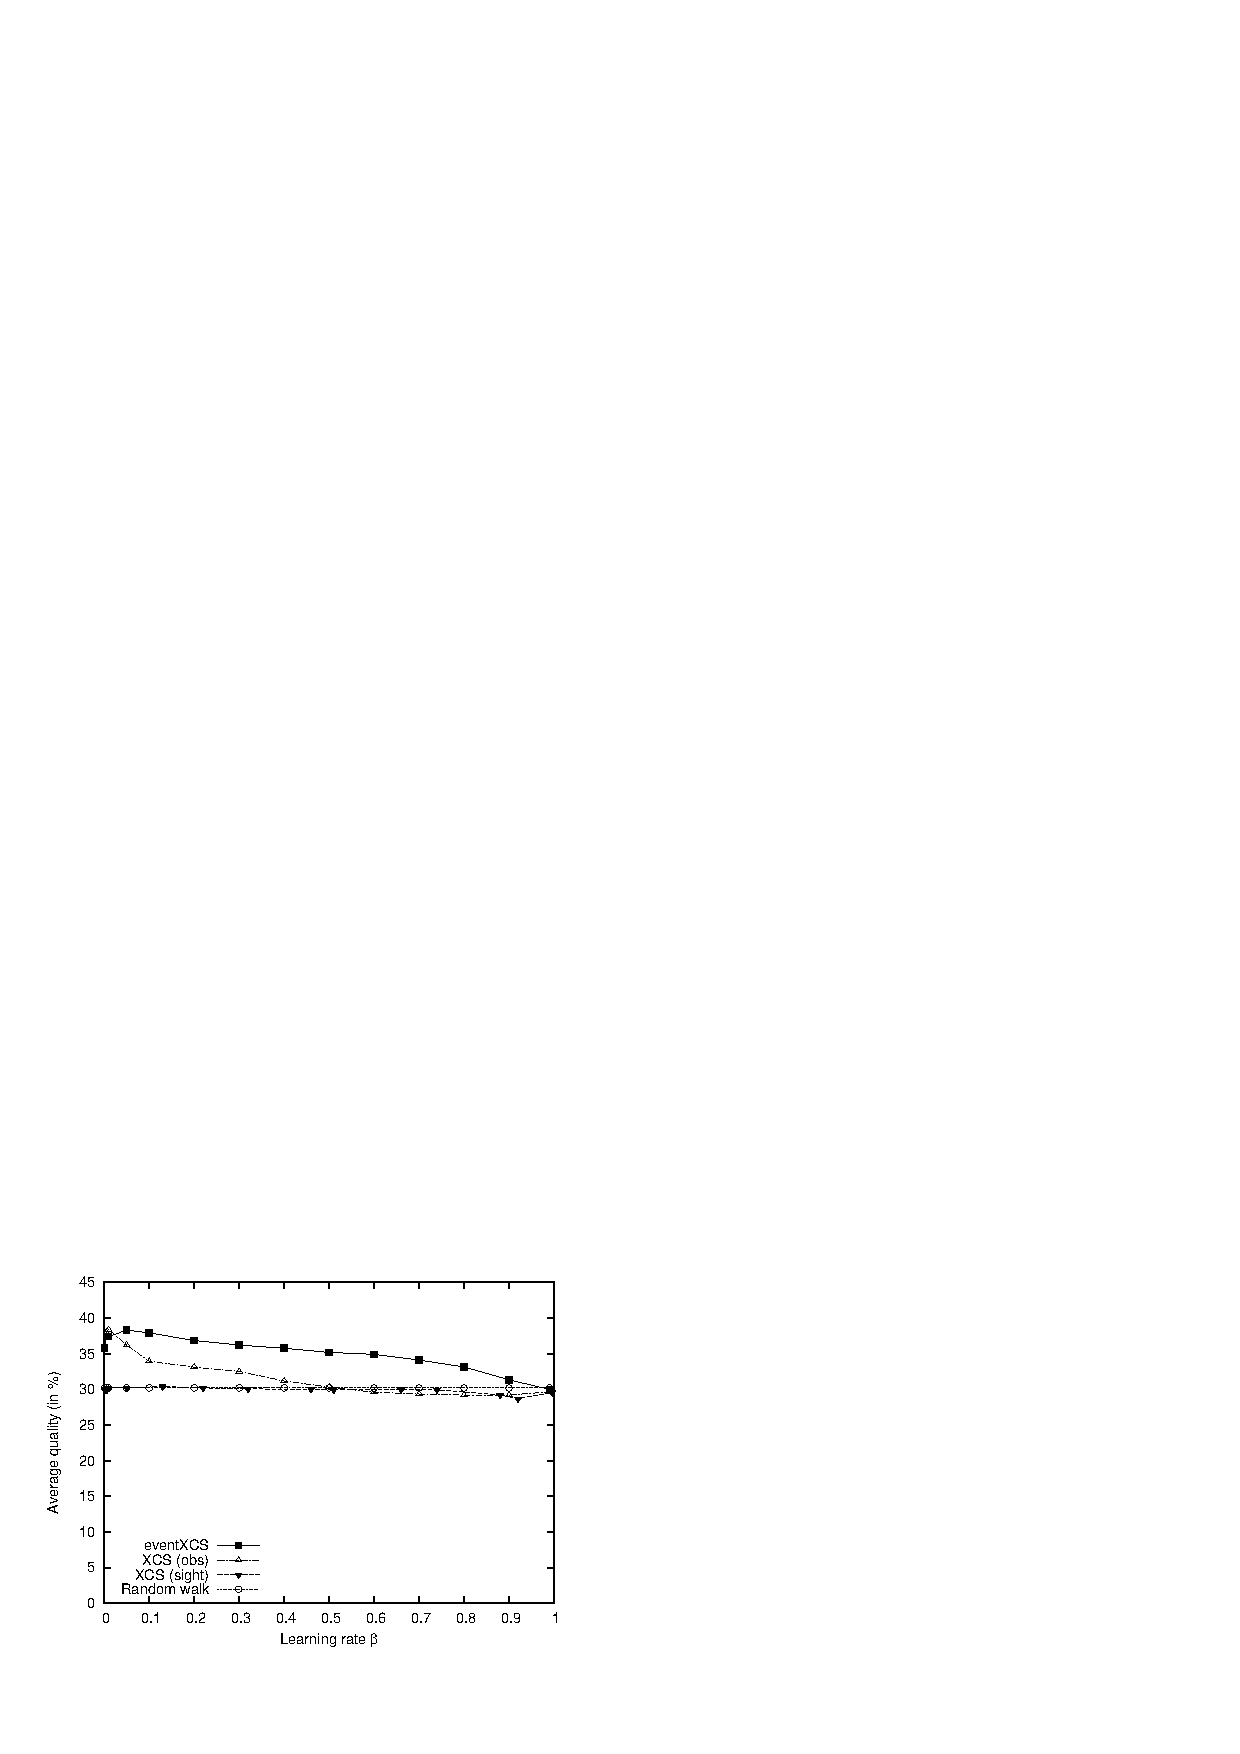
\includegraphics[width=0.24\textwidth]{plot_quality_learning-pillardir}}\hfill
	\subfigure[\emph{Pillar scenario} with a \emph{pre\-da\-tor-evading prey}]{
		\label{figure:learning_rate_pillar_intelligent}
		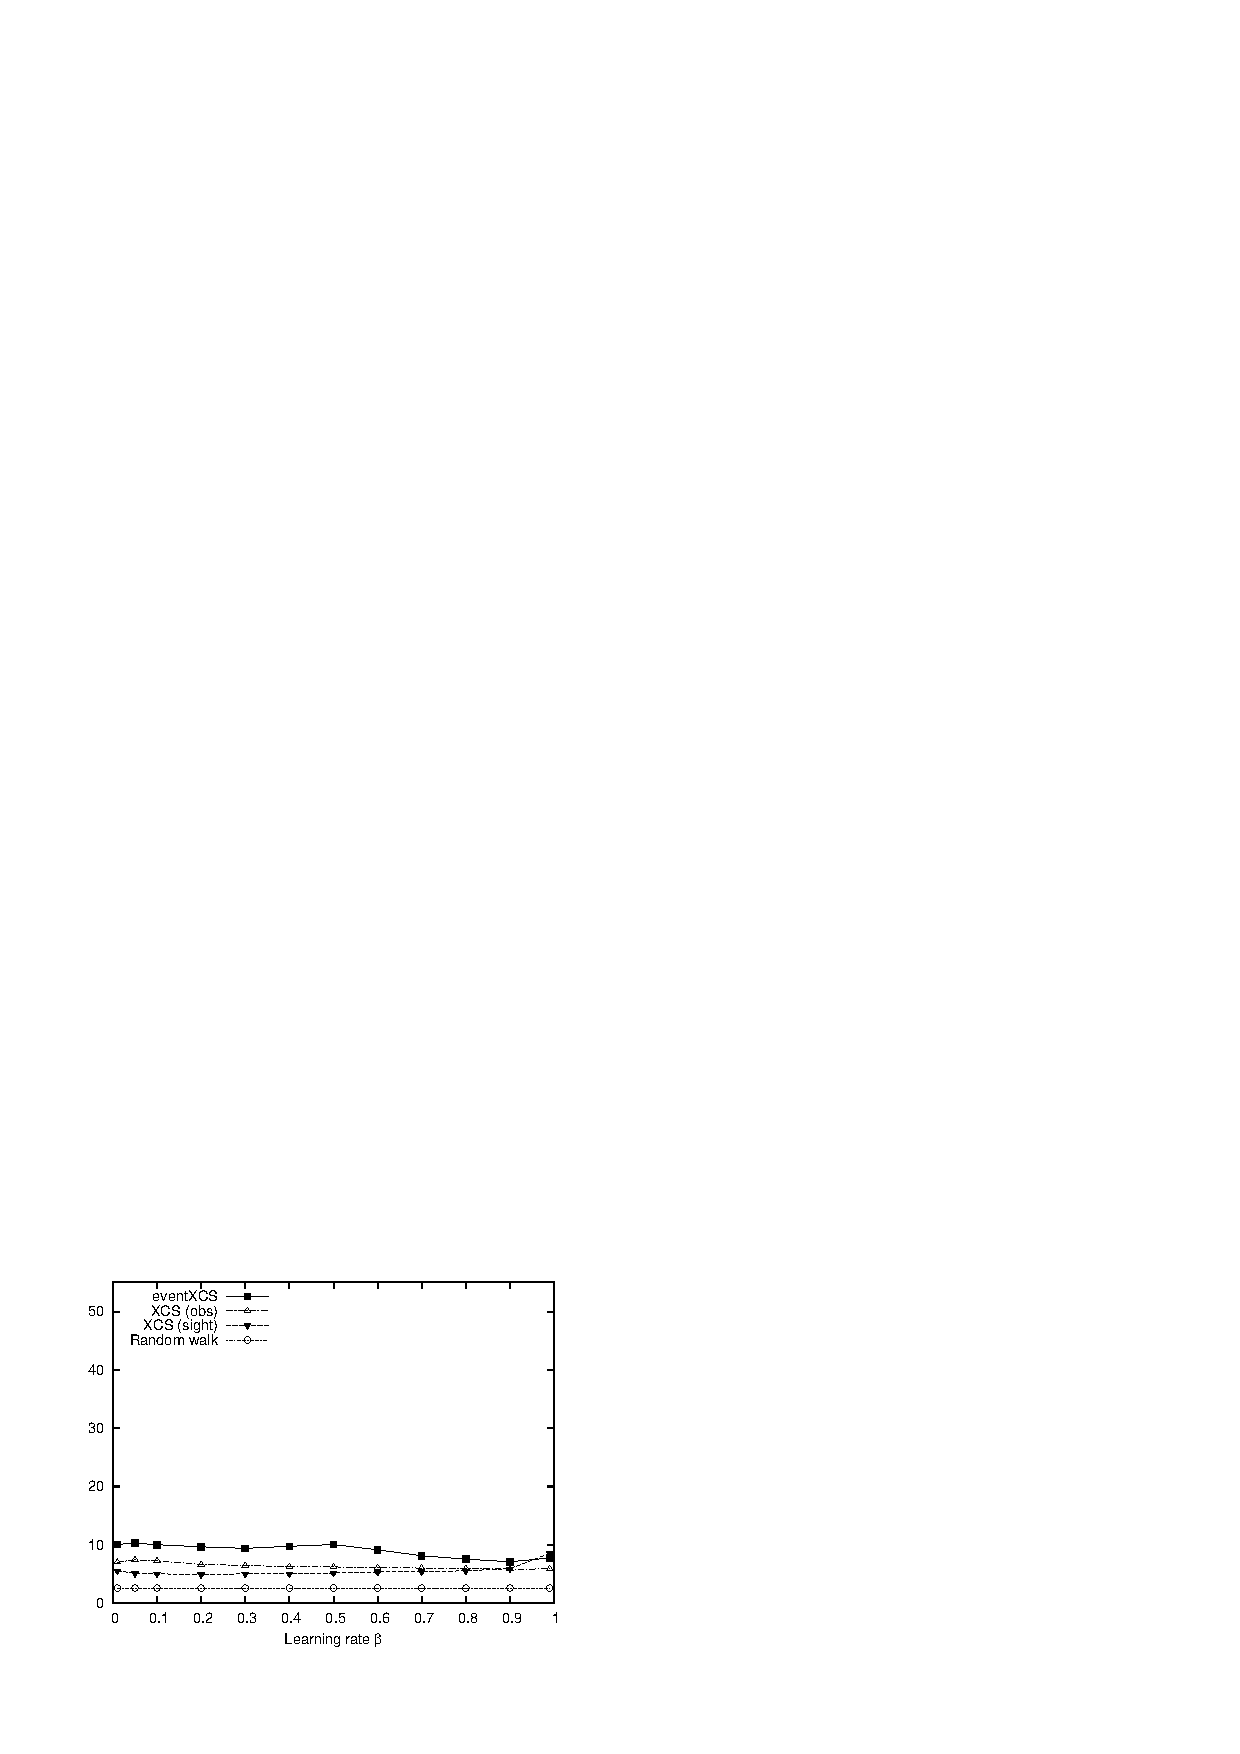
\includegraphics[width=0.24\textwidth]{plot_quality_learning-pillarint}}\hfill
	\subfigure[\emph{Random scenario} with an \emph{ob\-sta\-cle-evading prey}]{
		\label{figure:learning_rate_random_intelligent}
		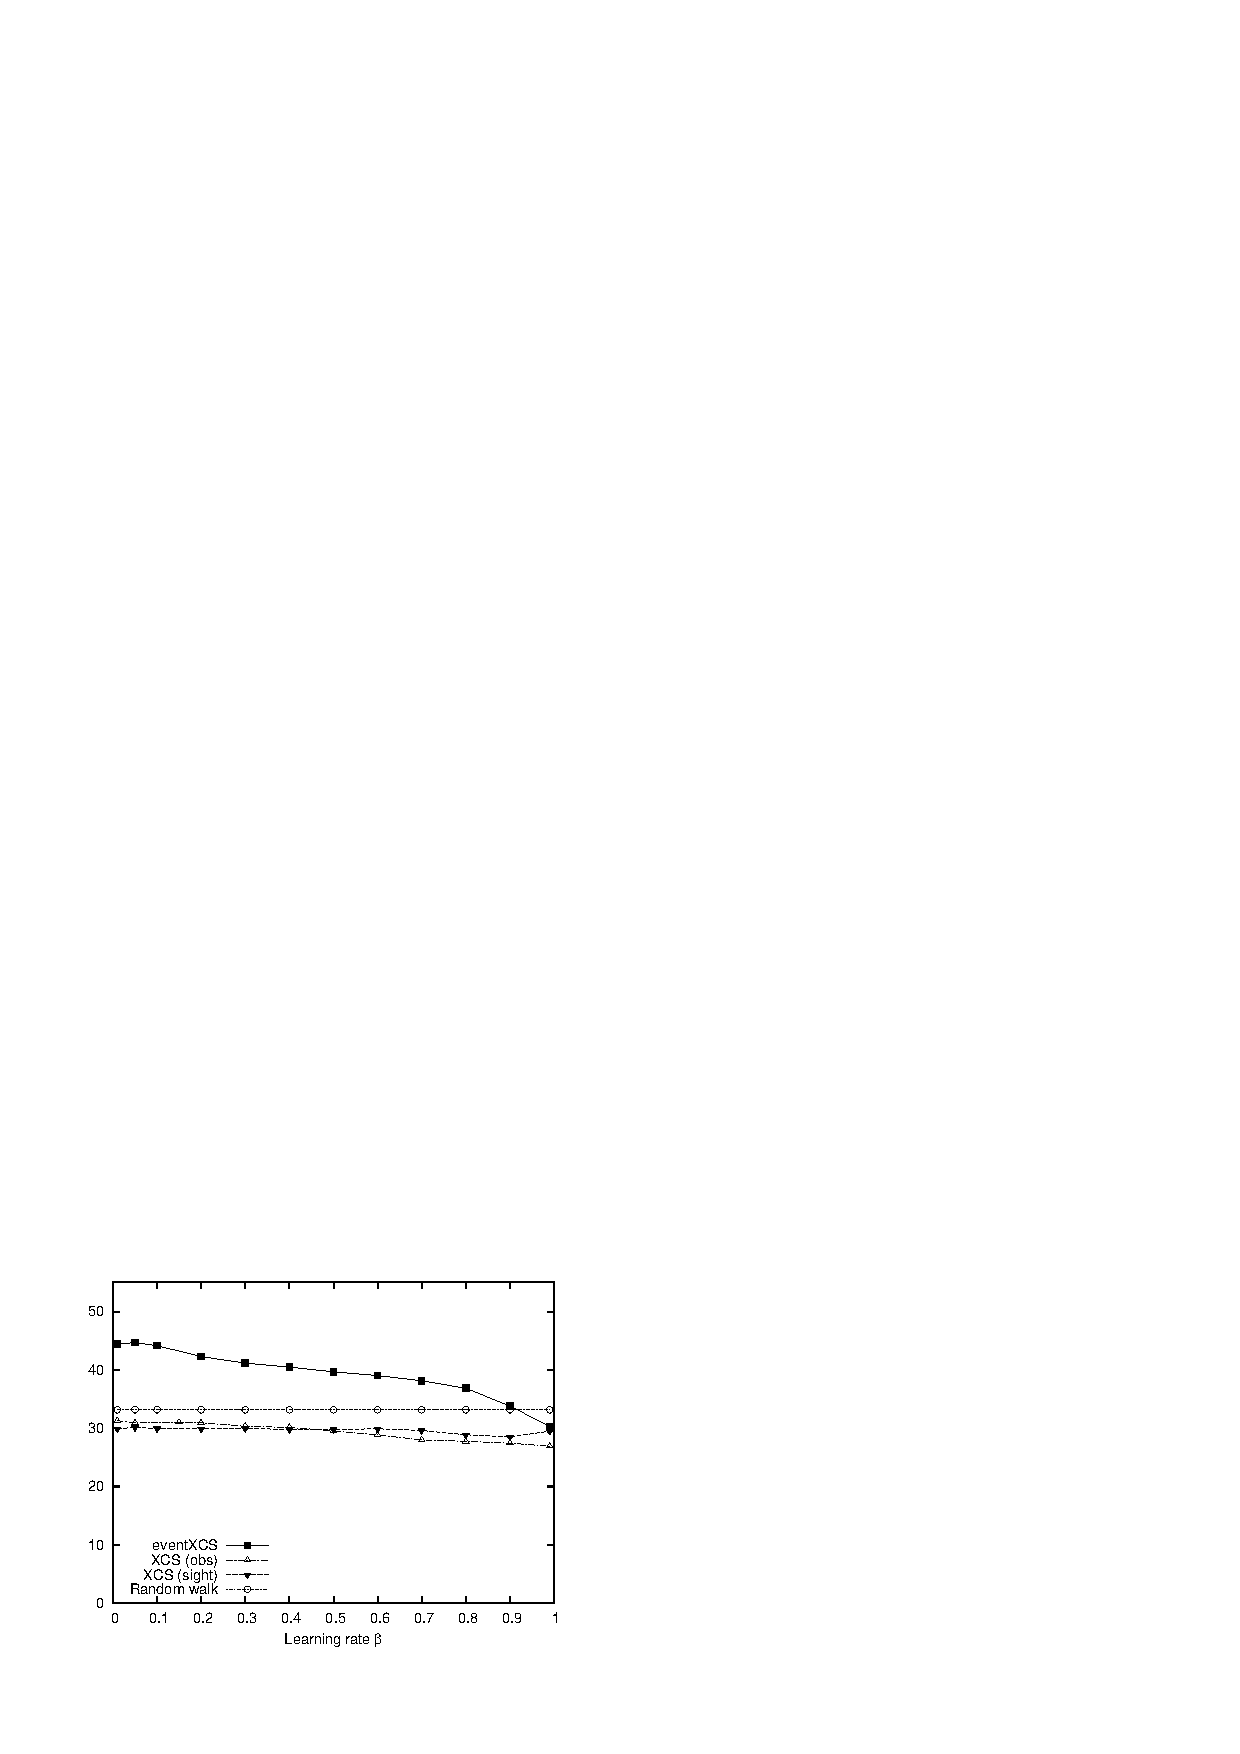
\includegraphics[width=0.24\textwidth]{plot_quality_learning-randdir}}\hfill
	\subfigure[\emph{Difficult scenario} with a \emph{blind\-ed prey}]{
		\label{figure:learning_rate_difficult}
		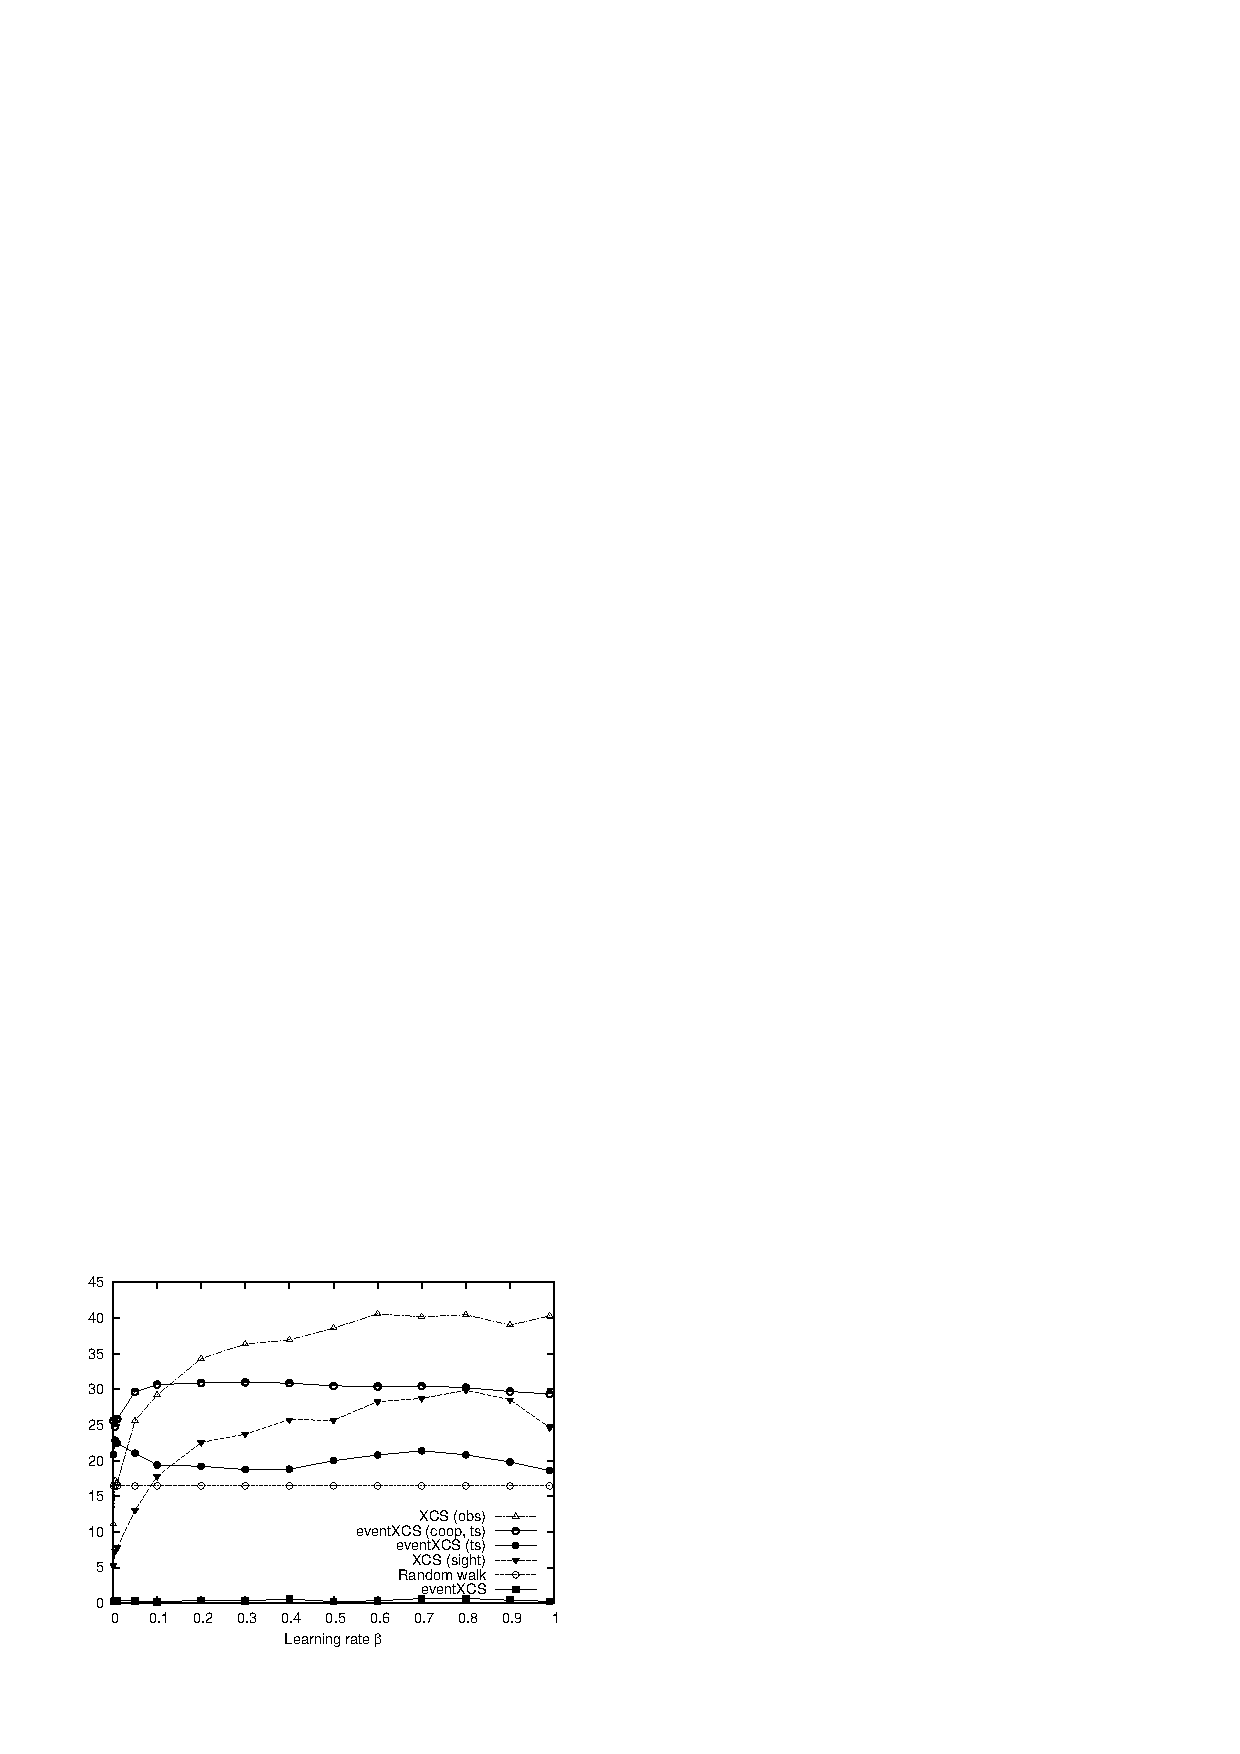
\includegraphics[width=0.24\textwidth]{plot_quality_learning-difficult}}
	\caption{\mathversion{bold}Comparison of different values for the learning rate $\beta$ for different XCS variants}
	\label{figure:learning_rate}
\end{figure*}

\begin{figure*}[ht]
  \subfigure[\emph{Pillar scenario} with an \emph{ob\-sta\-cle-evading prey}]{
  	\label{figure:experiment-pillardir}
  	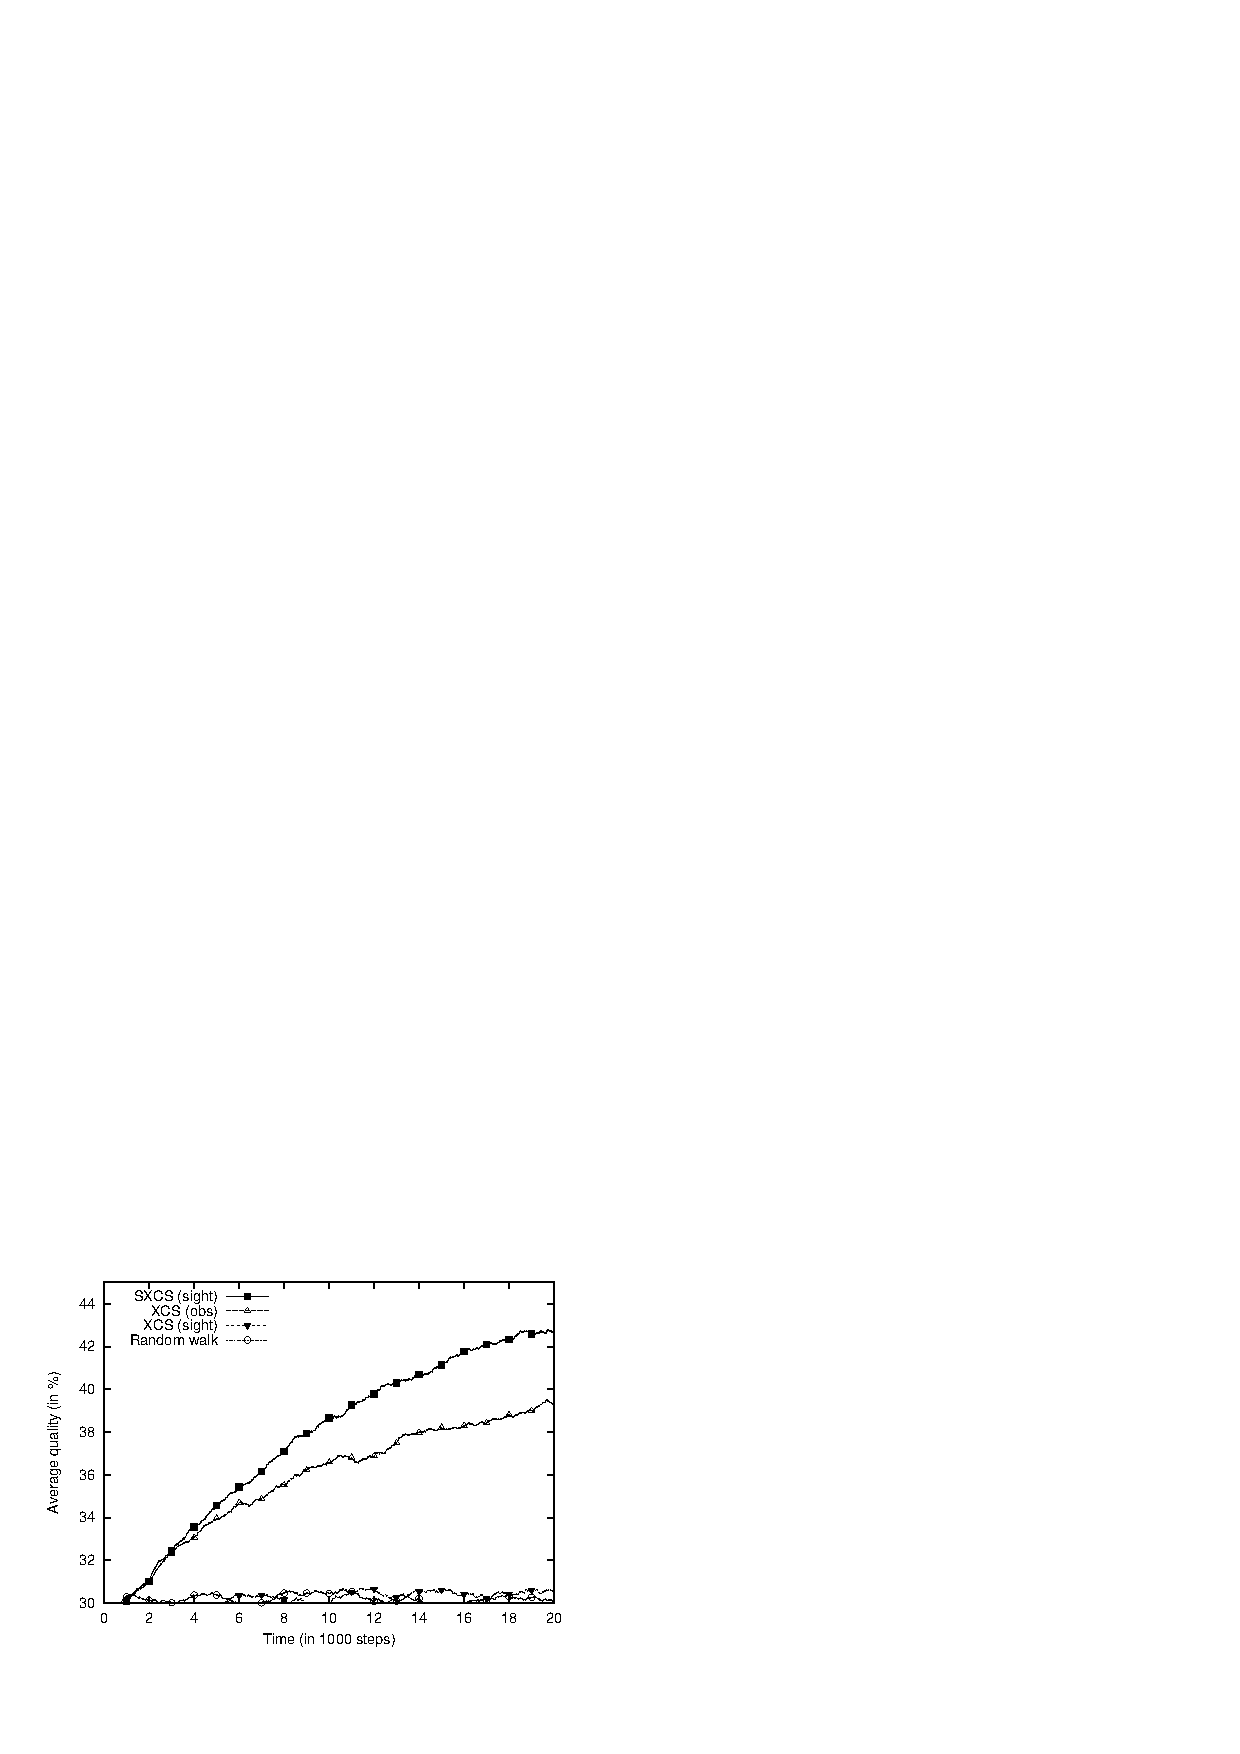
\includegraphics[width=0.24\textwidth]{plot_average_last_x_steps_goal_agent_observed-pillardir}}\hfill
  \subfigure[\emph{Pillar scenario} with a \emph{pre\-da\-tor-evading prey}]{
  	\label{figure:experiment-pillarint}
		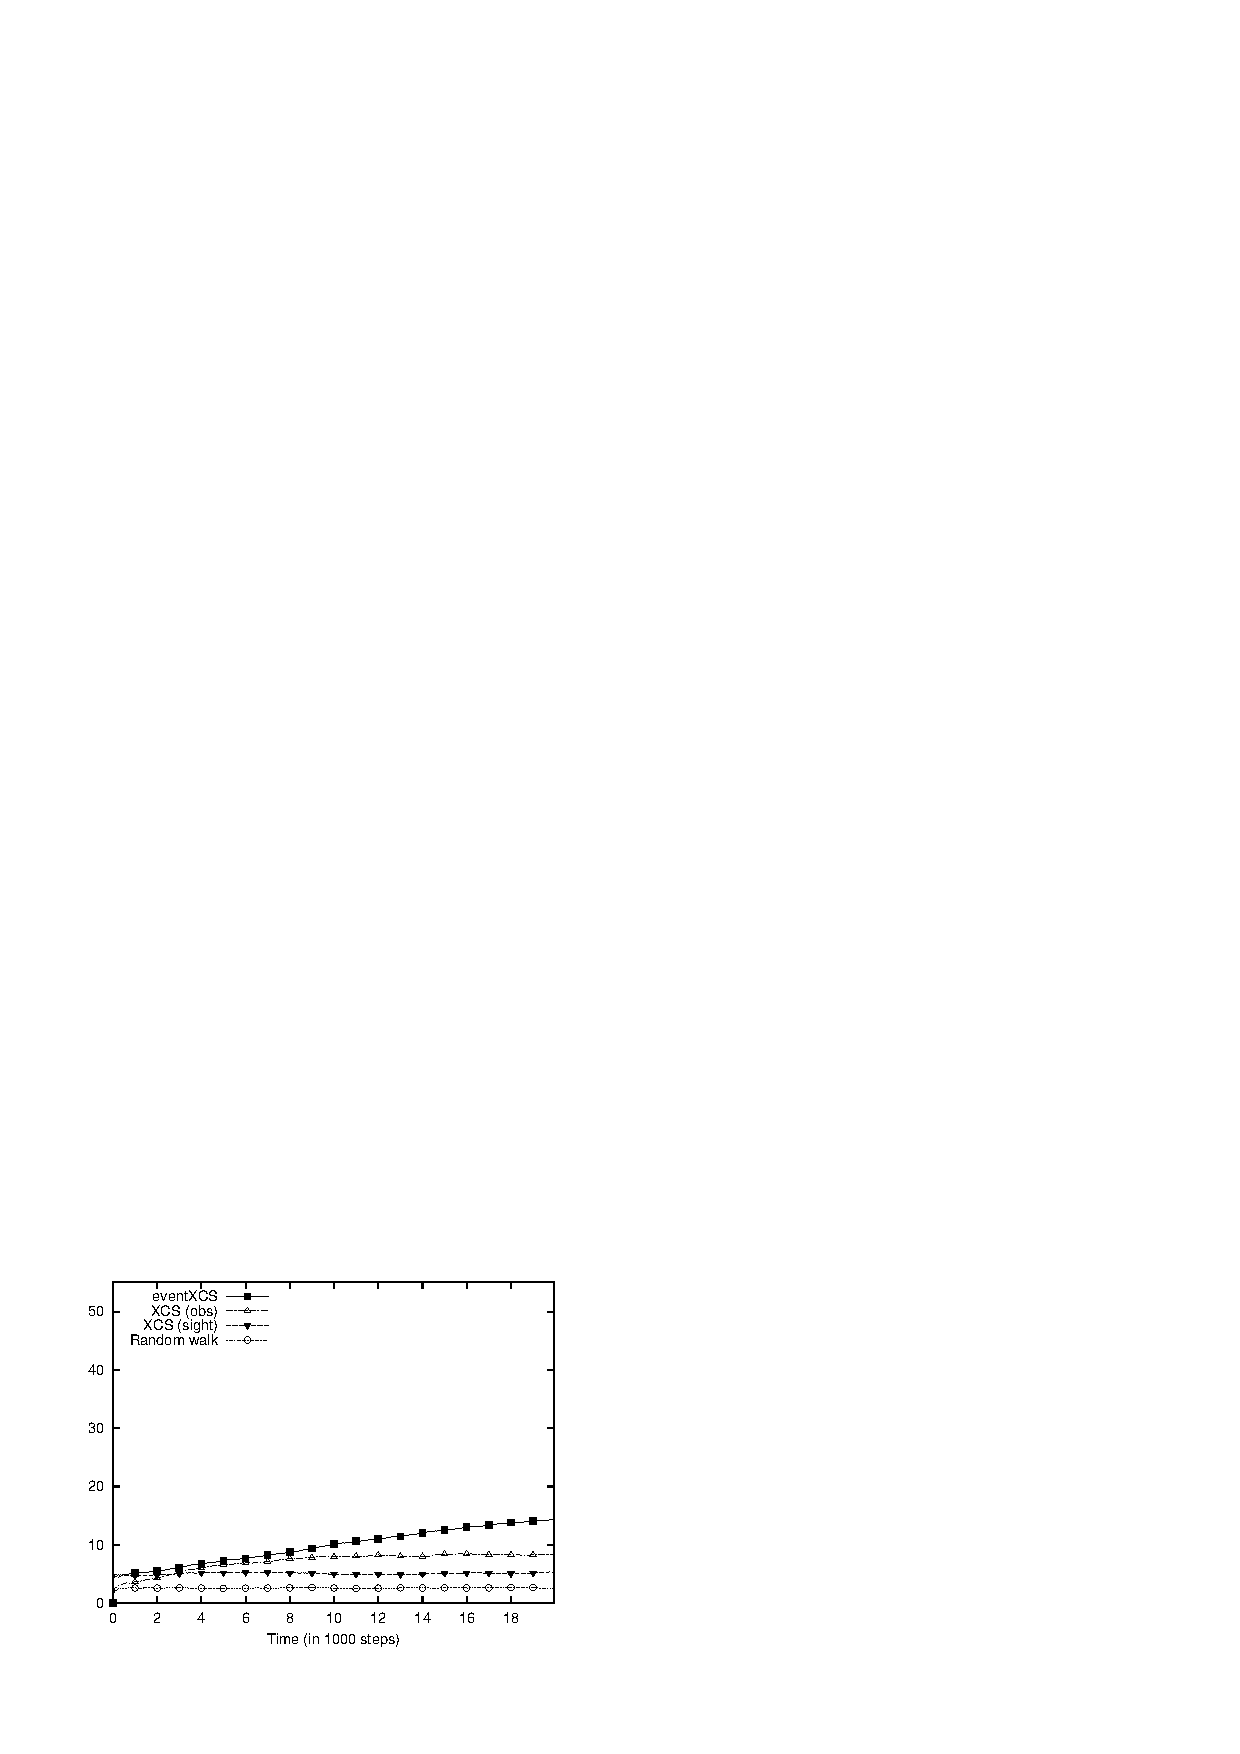
\includegraphics[width=0.24\textwidth]{plot_average_last_x_steps_goal_agent_observed-pillarint}}\hfill
  \subfigure[\emph{Random scenario} with an ob\-sta\-cle-evading prey]{
  	\label{figure:experiment-randdir}
		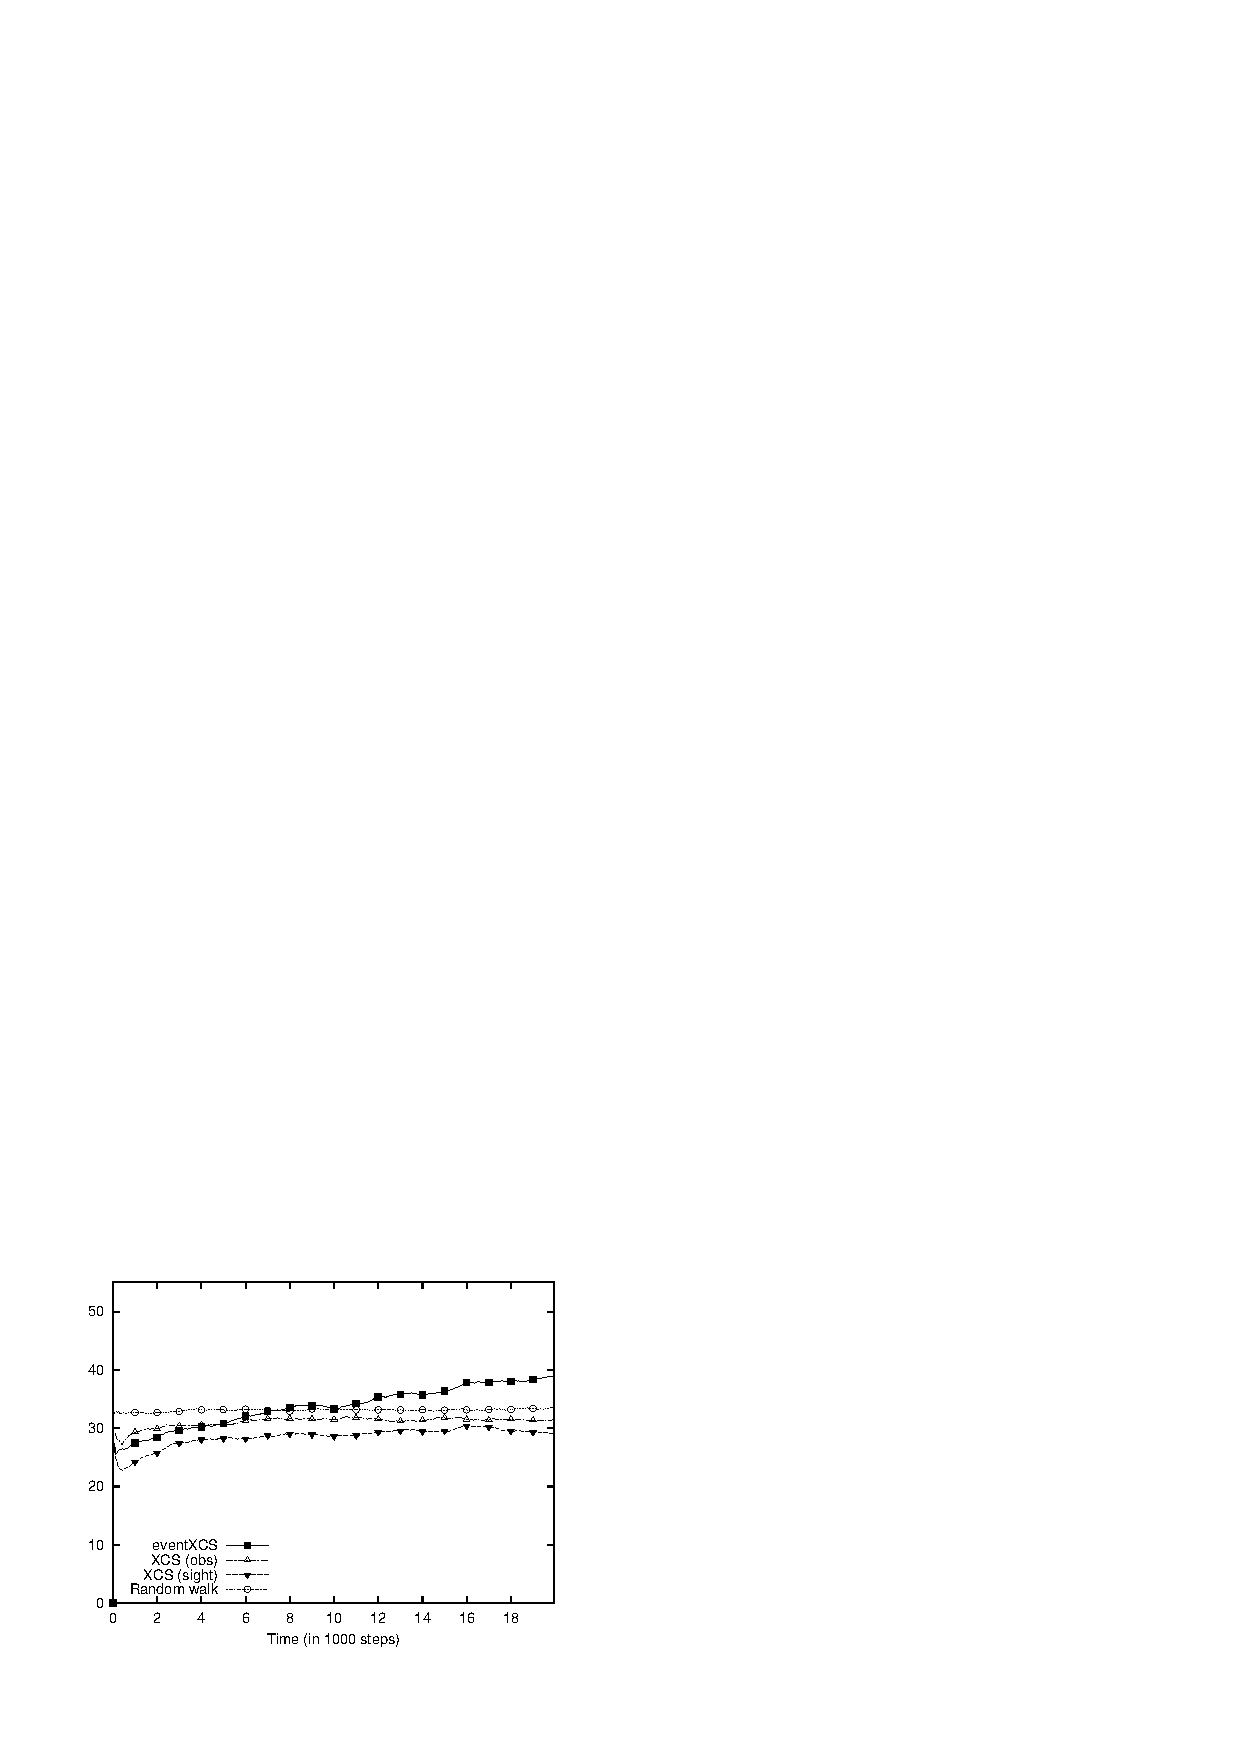
\includegraphics[width=0.24\textwidth]{plot_average_last_x_steps_goal_agent_observed-randdir}}\hfill
	\subfigure[\emph{Difficult scenario} with a \emph{blind\-ed prey}]{
		\label{figure:experiment-difficult}
		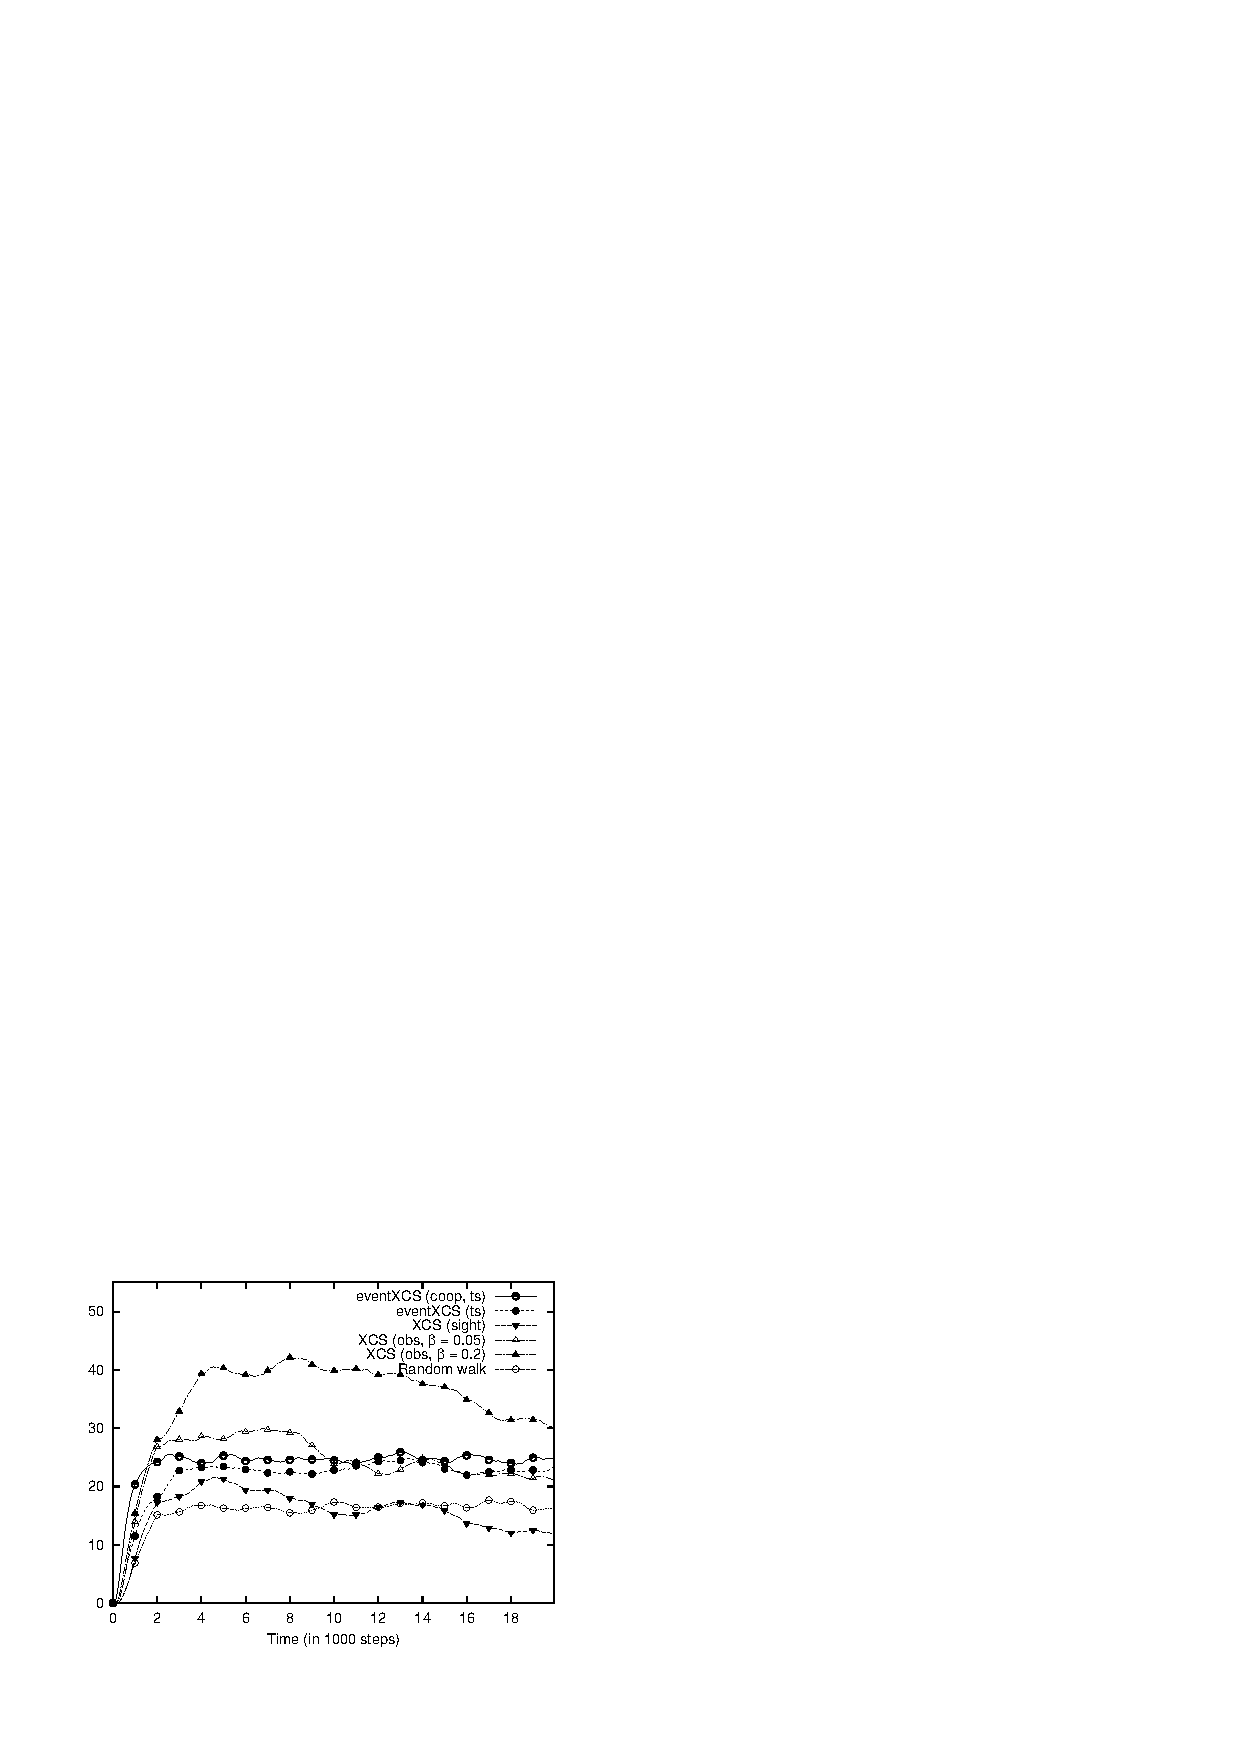
\includegraphics[width=0.24\textwidth]{plot_average_last_x_steps_goal_agent_observed-difficult}}
	\caption{\mathversion{bold}Comparison of the continuous average quality over time of different XCS variants}
	\label{figure:experiments}
\end{figure*}

\subsection{Discussion of Experimental Results}
\label{subsection:discussion-of-experimental-results}

As shown in Figures~\ref{figure:learning_rate} and \ref{figure:experiments}, \emph{XCS (sight)} is always inferior to \emph{XCS~(obs)}. Further tests on XCS plus different \emph{environmental reward functions} have led to the conclusion that XCS should not be combined with a reward function different to the global goal. Moreover, \emph{eventXCS} works well with strategies like \emph{selfish behavior (sight range)}, which is shown by the higher average quality of \emph{eventXCS} compared to \emph{XCS~(obs)} and an increased learning curve in the scenarios, depicted in Figures~\ref{figure:experiment-pillardir}, \ref{figure:experiment-pillarint}, and \ref{figure:experiment-randdir}. In the \emph{random scenario} with an obstacle-evading prey (see Figure~\ref{figure:experiment-randdir}), \emph{XCS} even shows no learning at all because of a relatively high percentage of wall collisions. Not depicted is the \emph{random scenario} with an predator-evading prey, the results are similar to the results of the \emph{pillar scenario} with the same type of prey.

% In addition, \emph{eventXCS} provides a significantly more stable learning, i.\,e., it shows no tendency of overlearning or unlearning, as shown in the \emph{random scenario} in Figure~\ref{figure:experiment-randdir}. Here, \emph{eventXCS} reaches significantly higher levels, while \emph{XCS (obs)} breaks down after 14,000 steps. To concluded, \emph{eventXCS} is clearly superior to \emph{XCS (obs)} in these three scenario configurations. 

Looking further on the \emph{difficult scenario}, it can be seen that \emph{eventXCS} clearly fails, no matter which \emph{learning rate} $\beta$ is used (see Figure~\ref{figure:learning_rate_difficult}). Since \emph{eventXCS} shares the same basic algorithm with \emph{XCS} and since the problem can be solved by choosing the classifiers more randomly using tournament selection (\emph{eventXCS~(ts)}), it points to a correctable flaw in the design of \emph{eventXCS}. Also including cooperative behavior (\emph{eventXCS~(coop,~ts)}) results in even better performance as the agents spread out more. While neither variant reaches the average quality level of \emph{XCS~(obs)}, they show a very stable learning, since \emph{XCS~(obs)} shows tendencies of over-learning or unlearning after 8\,000 steps or 14\,000 steps for $\beta = 0.2$ (see Figure~\ref{figure:experiment-difficult}). In general, it seems not surprising that \emph{XCS~(obs)} reaches better results than \emph{eventXCS}. \emph{XCS~(obs)} is designed to solve Maze scenarios, while \emph{eventXCS} has been modified to solve more open scenarios with a non-blinded prey, as investigated on the \emph{pillar} and the \emph{random scenario}. In summary, \emph{eventXCS} is clearly superior to \emph{XCS (obs)} in all four scenario configurations, it either reaches a better average quality or, with additional modifications, provides a similar quality with more stable learning.

% Alternative implementations of SXCS with \emph{tournament selection} on the other hand solve the problem but reach only a lower level as XCS with \emph{best selection} (see Figure~\ref{figure:experiment-difficult}). But as in the \emph{random scenario} with a predator-evading prey XCS seems to have problems with overlearning. Increasing the learning rate $\beta$ to $0.2$ increase the quality in short-term, but in long-term XCS still has problems while SXCS present a very stable learning curve. In connection with a collaborative base reward function SXCS is even able to outperform XCS in the long run.\\

% Figure~\ref{figure:experiment-heuristics} show a comparison between possible static strategies. Collaborative strategies have just a small advantage over simple greedy strategies.

% show the average percentage of time steps where the prey was in observation range (each averaged over the last 2000 steps). With an predator-evading prey SXCS clearly outperforms XCS, while in the case with the obstacle-evading prey both variants show a similar learning curve. In all cases increasing the base reward function for XCS from observation range to sight range resulted in worse results.\\
%The case with an obstacle-evading prey in the \emph{random scenario} is not displayed, none of the XCS variants are able to gain a significant advantage over a ``random walk'' strategy.

% In Section~\ref{section:experimental-results} it was shown that SXCS outperforms XCS in scenarios with few obstacles. This was mainly due to the fact that XCS is unable to handle base reward functions that differ from the global goal and because XCS seems to have problems reaching a stable level, possibly due to overlearning. 
%SXCS with \emph{best selection} showed serious problems in the \emph{difficult scenario} while it was able manage the problem with a more random \emph{tournament selection}. This points to a correctable flaw in the design of the algorithm (probably with the \emph{neutral events}). But other than XCS SXCS \emph{can} handle advanced base reward functions, e.g. with a collaborative element (evading other agents) which significantly helps for example in the \emph{difficult scenario} though this is probably due to the fact that it simply encourages agents to move away from other agents, explore the grid and move through the openings. But in the end SXCS was designed to follow and observe a moving prey, the \emph{difficult scenario} is more like a labyrinth where finding the prey in the first place is important.
